\documentclass[lang=cn,11pt,marginpar=margintrue]{elegantbook}%
%\syntaxonly
\newcommand{\daan}[1]{\hfill\hyperref[#1]{
\includegraphics[width=1pc]{daan}}}
\newcommand{\xiahua}[1]{ \underline{\hspace{#1 pc}} }
\newcommand{\dd}{\zt{d}}
\newcommand{\zt}[1]{\,\mathrm{#1}}
\newcommand{\NN}{\mathrm{N}}
\newcolumntype{Z}{>{\centering\arraybackslash}X}
%\setlist[enumerate]{leftmargin=*}
% title info
\title{《电机学》题库}
\subtitle{$2017-2019$ 汇总\footnote{老师所给题的汇总}}
% bio info
\author{死抠\footnote{江理学习资料库: \url{https://github.com/sikouhjw/jxust-Learning-database}}}
\institute{$\mathrm{miu}$ 组织}
\date{\today}
% extra info
\version{1.00}
\extrainfo{Victory won\rq t come to us unless we go to it. --- M. Moore}
\logo{logo.png}
\cover{cover.jpg}
\begin{document}

\maketitle
\tableofcontents
\mainmatter
\hypersetup{pageanchor=true}
% add preface chapter here if needed
\chapter{电机题库}
说明: 从未考虑手机用户, 请使用电脑查看本文件, 推荐使用 \href{https://www.sumatrapdfreader.org/free-pdf-reader.html}{ $\zt{SumatraPDF}$ } 查看.

文件中彩色部分大多数为交叉引用(即点击后会跳转), {\bfseries点击 
\includegraphics[width=0.03\textwidth]{daan} 符号, 可以查看答案}.
\section{填空题}
\begin{enumerate}
	\item (17,19)直流电动机励磁方式有\xiahua{3.5}、\xiahua{3.5}、\xiahua{3.5}和\xiahua{3.5}.\daan{tk:1}
	\item (17,18,19)在直流发电机中, 电枢绕组中的感应电动势是\xiahua{4}电动势, 电刷间的感应电动势是\xiahua{4}电动势.\daan{tk:2}
	\item (17,18,19)他励直流电动机有\xiahua{4}、\xiahua{4}和\xiahua{4}制动方式, 有\xiahua{4}和\xiahua{4}反接制动方法.\daan{tk:3}
	\item (17,18,19)笼形感应电动机降压起动的方法有\xiahua{4}、\xiahua{4}、\xiahua{4}和\xiahua{4}四种.\daan{tk:4}
	\item (17,18,19)变压器/感应电动机等效电路中的 $X_{\mathrm{m}}$ 对应于\xiahua{3}, $R_{\mathrm{m}}$ 是表示\xiahua{3}, $Z_{\mathrm{m}}$ 是表示\xiahua{3}.\daan{tk:5}
	\item (17,18,19)绕线式三相异步电动机, 如果电源电压一定, 转子回路电阻适当增大, 则起动转矩\xiahua{4}, 最大转矩\xiahua{4}, 临界转差率\xiahua{4}, 转速\xiahua{4}, 定子电流\xiahua{4}.\daan{tk:6}
	\item (17,18,19)异步电动机和变压器主磁场性质不同, 异步电动机气隙中的磁场为
	
	\xiahua{4}磁场, 而变压器为\xiahua{4}磁场.\daan{tk:7}
	\item (17,18,19)感应电机带恒转矩负载进行变频调速时, 保证 $\frac{U_1}{f_1}$ 为常数的目的在于使电机的\xiahua{4}和\xiahua{4}保持不变.\daan{tk:8}
	\item (17,18,19)感应电机星形—三角形降压起动时, 起动电流和起动转矩降为直接起动时的\xiahua{4}倍.\daan{tk:9}
	\item (18,19)并励直流发电机自励建压的条件有\xiahua{4}、\xiahua{8}和\xiahua{4}.\daan{tk:10}
	\item (17,18,19)直流发电机的绕组常用的有\xiahua{4}和\xiahua{4}两种形式, 其各自的特点分别是\xiahua{8}和\xiahua{8}.\daan{tk:11}
	\item (17,18,19)他励直流电动机的固有机械特性是指在\xiahua{4}、\xiahua{4}, 电枢回路不串\xiahua{4}条件下,\xiahua{4}和\xiahua{4}的关系.\daan{tk:12}
	\item (18,19)通常直流电动机的起动方法有\xiahua{4}和\xiahua{4}两种.\daan{tk:13}
	\item (17,18,19)当电动机的转速超过\xiahua{4}时, 会出现回馈制动.\daan{tk:14}
	\item (17,18,19)一个三相对称交流绕组, 三相对称交流电流, 其合成磁动势为\xiahua{4}磁动势, 旋转方向由\xiahua{4}决定, 转速为\xiahua{4}.\daan{tk:15}
	\item (18,19)三相异步电动机等效电路中的附加电阻是模拟\xiahua{4}的等值电阻.\daan{tk:16}
	\item (17,18,19)拖动恒转矩负载运行的三相异步电动机, 其转差率 $s$ 在\xiahua{4}范围内时, 电动机都能稳定运行.\daan{tk:17}
	\item (18,19)深槽与双笼型异步电动机由于\xiahua{4}, 起动转矩大.\daan{tk:18}
	\item (17,18,19)改变\xiahua{4}或改变\xiahua{4}均能使直流电动机反转.\daan{tk:19}
	\item (17,18,19)他励直流电动机\xiahua{4}和\xiahua{4}, 都可做到无级调速.\daan{tk:20}
	\item (17,19)直流发电机电磁转矩的方向和电枢旋转方向\xiahua{4}, 直流电动机电磁转矩的方向和电枢旋转方向\xiahua{4}.\daan{tk:21}
	\item (17,18,19)一台接到电源频率固定的变压器, 在忽略漏阻抗压降条件下, 其主磁通的大小决定于\xiahua{4}的大小, 而与磁路的\xiahua{4}和\xiahua{4}基本无关, 其主磁通与励磁电流成\xiahua{4}关系.\daan{tk:22}
	\item (17,19)一个脉振磁动势可以分解为两个\xiahua{4}和\xiahua{4}相同, 而\xiahua{4}相反的旋转磁动势.\daan{tk:23}
	\item (17,19)三相异步电动机的过载能力是指\xiahua{4}.\daan{tk:24}
	\item (17,19)直流发电机主磁极磁通产生感应电动势存在于\xiahua{4}绕组中.\daan{tk:25}
	\item (17,18,19)电力拖动系统运动方程式中的 $GD^2$ 反映了\xiahua{8}.\daan{tk:26}
	\item (17,19)直流电动机采用降低电源电压的方法起动, 其目的是为了\xiahua{4}.\daan{tk:27}
	\item (17,19)变压器空载电流小的原因是\xiahua{8}.\daan{tk:28}
	\item (17,19)三相异步电动机在运行中, 把定子两相反接, 则转子的转向会\xiahua{4}.\daan{tk:29}
	\item (19)写出三相感应电动机的功率平衡方程\xiahua{8}和转矩平衡方程
	
	\xiahua{8}.\daan{tk:30}
	\item (19)写出三相感应电动机与等值电路有关的基本方程组\xiahua{8}.\daan{tk:31}
	\item (18)变压器空载电流大小与励磁阻抗大小之间的关系是\xiahua{4}.\daan{tk:32}
	\item (18)变压器铁心导磁性能越好, 其励磁电抗越\xiahua{4}, 励磁电流越\xiahua{4}.\daan{tk:33}
	\item (18)三相异步电动机电源电压一定, 当负载转矩增加, 则转速\xiahua{4}, 定子电流\xiahua{4}.\daan{tk:34}
	\item (18)容量为几个千瓦时的直流电动机不能直接起动而三相笼型异步电动机却可以直接起动的原因是\xiahua{8}.\daan{tk:35}
	\item (17)直流电动机直接起动的不利影响有\xiahua{8}.\daan{tk:36}
	\item (18)三相异步电动机空载运行时, 电动机的功率因数很低的原因是\xiahua{5}.\daan{tk:37}
	\item (18)串励直流电动机运行和传动有特殊要求:\xiahua{8}, 并励直流电动机运行和传动有特殊要求:\xiahua{8}.\daan{tk:38}
	\item (18)他励直流电动机, 降低电源电压调速属\xiahua{3}调速方式, 适合拖动\xiahua{3}负载.\daan{tk:39}
	\item (17)直流电机的电磁转矩是由\xiahua{4}和\xiahua{4}共同作用产生的.\daan{tk:40}
	\item (17)直流电动机电动势的方向和电流的方向\xiahua{4}, 电磁转矩的方向和转向\xiahua{4}.\daan{tk:41}
	\item (17)常见生产机械负载转矩特性有\xiahua{5}、\xiahua{5}、\xiahua{5}、\xiahua{5}.\daan{tk:42}
	\item (17)一台控制用单相变压器, 额定容量 $S_{\NN}=100\zt{V\cdot A}$ ,  额定电压 $U_{1\NN}/U_{2\NN}=380/36\zt{V}$ , 它的原边额定电流为\xiahua{4}, 副边额定电流为\xiahua{4}.\daan{tk:43}
	\item (17)三相异步电动机降低定子电压, 则最大转矩 $T_{\mathrm{m}}$ \xiahua{2}, 起动转矩 $T_Q$ \xiahua{2}, 临界转差率 $S_{\mathrm{m}}$ \xiahua{2}.\daan{tk:44}
	\item (17)一台 $6$ 极三相异步电动机接于 $50\zt{Hz}$ 的三相对称电源, 其 $S=0.05$ , 则此时转子转速为\xiahua{4}, 定子旋转磁通势相对于转子的转速为\xiahua{4}.\daan{tk:45}
	\item (17)同步电动机在过励磁时呈\xiahua{4}负载, 它能提高\xiahua{4}.\daan{tk:46}
	\item (17)交直流电机的三个基本组成部分是\xiahua{3}、\xiahua{3}和\xiahua{3}.\daan{tk:47}
	\item (17)直流电动机交轴电枢反应将使\xiahua{8}发生畸变, 使\xiahua{4}偏离几何中线, 磁路饱和时, 使每极\xiahua{4}减小.\daan{tk:48}
	\item (17)单叠和单波绕组, 极对数均为 $p$ 时, 并联支路数分别是\xiahua{2}和\xiahua{2}.\daan{tk:49}
	\item (17)三相异步电动机带恒转矩负载运行,  如果电源电压下降,  当电动机稳定运行后, 此时电动机的电磁转矩\xiahua{4}.\daan{tk:50}
	\item (17)电力拖动系统静态转矩的折算原则是\xiahua{8}, 转动惯量的折算原则是\xiahua{8}.\daan{tk:51}
	\item (17)改变直流电动机的端电压的调速方法适合拖动恒\xiahua{2}负载, 改变主磁极磁通调速方法适合拖动恒\xiahua{2}负载.\daan{tk:52}
	\item (17)感应电动机改变同步转速的调速方式有\xiahua{2}和\xiahua{2}两种.\daan{tk:53}
	\item (17)隐极式同步电动机气隙\xiahua{2}, 只存在\xiahua{2}电磁转矩, 而凸极式同步电动机气隙\xiahua{3}, 其电磁转矩中包含\xiahua{6}和\xiahua{6}两部分.\daan{tk:54}
	\item (17)直流发电机电刷顺转向移动时, 顺轴电枢反应的结果是\xiahua{2}.\daan{tk:55}
	\item (17)他励直流电动机正向回馈制动时, $E_a$ , $U$ , $n$ 的关系为 $E_a$ \xiahua{1} $U$ , $n$ \xiahua{1} $n_0$ .\daan{tk:56}
	\item (17)电力拖动系统平衡状态稳定运行的条件是\xiahua{4}.\daan{tk:57}
	\item (17)假设并励直流发电机正转时能自励, 电机输出端电压为 $+U$ , 则电机反转也能自励的条件是\xiahua{10}.\daan{tk:58}
	\item (17)改善直流电机换向的方法有\xiahua{4}和\xiahua{4}两种.\daan{tk:59}
	\item (17)变压器的折算方法是\xiahua{20}, 折算原则是\xiahua{8}.\daan{tk:60}
	\item (17)感应电动机转子回路串入电阻后, 机械特性上\xiahua{2}不变.\daan{tk:61}
	\item (17)变压器空载试验一般在\xiahua{2}侧进行, 变压器空载试验目的是\xiahua{6}
	
	\xiahua{30}.\daan{tk:62}
	\item (17)同步电机是\xiahua{20}的电机, 其转速与极对数之间的关系是\xiahua{4}.\daan{tk:63}
\end{enumerate}
\section{画图题}
\begin{enumerate}
	\item (17,18,19)画出并励直流电动机的固有机械特性和人为机械特性曲线.\daan{ht:1}
	\item 异步电动机的机械特性和等效电路.\daan{ht:2}
	\item 变压器的等效电路.\daan{ht:3}
	\item \label{h:3}画出\hyperref[tu:1]{图示}三相变压器连接法的相量图, 并据其标出连接组号.\daan{ht:4}
			\begin{figure}[htbp]
				\centering
				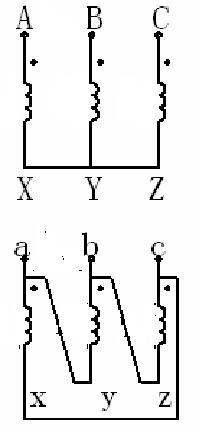
\includegraphics[width=0.15\textwidth]{tu1.png}
				\qquad
				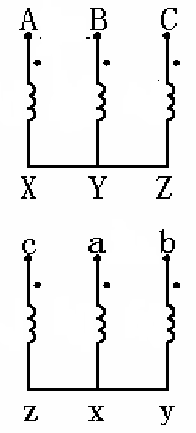
\includegraphics[width=0.15\textwidth]{tu7.png}
				\qquad
				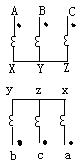
\includegraphics[width=0.15\textwidth]{tu9.png}
				\qquad
				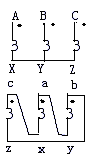
\includegraphics[width=0.15\textwidth]{tu10.png}\\
				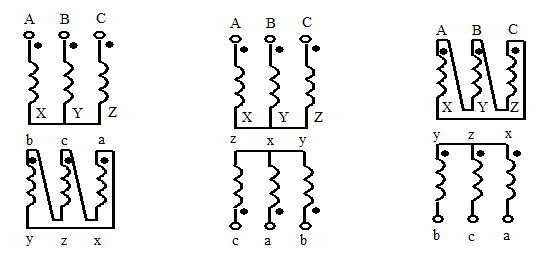
\includegraphics[width=0.8\textwidth]{tu8.png}
				\caption{画图题~\ref{h:3}~的图}\label{tu:1}
				\end{figure}
	\item (19)三相感应电动机的能流图.\daan{ht:5}
\end{enumerate}

\section{计算题}
\begin{enumerate}
	\item (17,18)一台他励直流电动机, 铭牌数据如下: $P_{\NN}=60\zt{kW}$ , $U_{\NN}=220\zt{V}$ , $I_{\NN}=305\zt{A}$ , $n_{\NN}=1000\zt{r/min}$ . 试求:
		\begin{enumerate}
			\item 固有机械特性.
			\item $R_{C}=0.5\Omega$ 的人为机械特性.\daan{js:1}
		\end{enumerate}
	\item (17,18,19)电力拖动系统的传动机构如图~\ref{tu:4}~所示, 已知: $n_1=2500\zt{r/min}$ , $n_2=1000\zt{r/min}$ , $n_3=500\zt{r/min}$ , $GD_1^2=8\zt{kg\cdot m^2}$ , $GD_2^2=25\zt{kg\cdot m^2}$ , $GD_3^2=75\zt{kg\cdot m^2}$ , 负载转矩 $T_Z=10\zt{kg\cdot m}$ , 电磁转矩 $T=3\zt{kg\cdot m}$ , 试求:
		\begin{enumerate}
			\item 生产机械轴的平均加速度为多少?
			\item 要加装 $62.5\zt{kg\cdot m^2}$ 的飞轮, 以使生产机械轴的平均加速度为 $3 \zt{r/(min\cdot s)}$ , 此飞轮应装在哪个轴合适?\daan{js:2}
		\end{enumerate}
		\begin{figure}[htbp]
			\centering
			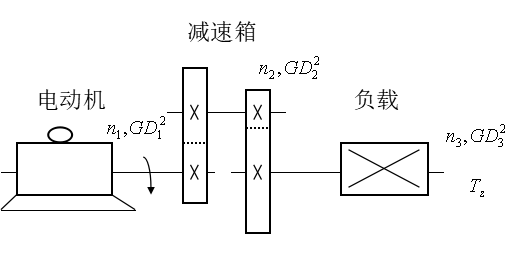
\includegraphics[width=0.7\textwidth]{tu4}
			\caption{传动机构图}\label{tu:4}
		\end{figure}
	\item (17,18,19)一台他励直流电动机, 额定数据为: $P_{\NN}=1.1\zt{kW}$ , $U_{\NN}=110\zt{V}$ , $I_{\NN}=13\zt{A}$ , $n_{\NN}=1500\zt{r/min}$ , 电枢回路电阻 $R_a=1\Omega$ . 计算:
		\begin{enumerate}
			\item 额定电磁转矩.
			\item 额定输出转矩.
			\item 空载转矩.
			\item 理想空载转矩.
			\item 实际空载转矩.\daan{js:3}
		\end{enumerate}
	\item (17,18,19)一台他励直流电动机数据为: $P_{\NN}=7.5\zt{kW}$ , $U_{\NN}=110\zt{V}$ , $I_{\NN}=79.84\zt{A}$ , $n_{\NN}=1500\zt{r/min}$ , 电枢回路电阻 $R_a=0.1014\Omega$ , 求:
		\begin{enumerate}
			\item $U=U_{\NN}$ , $\varPhi=\varPhi_{\NN}$ 条件下, 电枢电流 $I_a=60\zt{A}$ 时转速是多少?
			\item $U=U_{\NN}$ 条件下, 主磁通减少 $15\%$ , 负载转矩为 $T_{\NN}$ 不变时, 电动机电枢电流与转速是多少?
			\item $U=U_{\NN}$ , $\varPhi=\varPhi_{\NN}$ 条件下, 负载转矩为 $0.8T_{\NN}$ , 转速为 $800\zt{r/min}$ , 电枢回路应串入多大电阻?\daan{js:4}
		\end{enumerate}
	\item (19)一台 $S_{\NN}=100\zt{kV\cdot A}$ , $U_{1\NN}/U_{2\NN}=6/0.4\zt{kV}$ , $\mathrm{Yy}0$ 连接的三相变压器, $I_0^*=6.5\% $ , $P_0=600\zt{W}$ , $u_{S_{\NN}}^*=5\%$ , $P_{S_{\NN}}=1800\zt{W}$ , 试求:
		\begin{enumerate}
			\item 近似等效电路参数标么值.
			\item 满载及 $\cos\varPhi_2=0.8(\text{滞后})$ 时的二次端电压和效率.
			\item 产生最大效率时的负载电流及 $\cos\varPhi_2=0.8(\varPhi_2>0^\circ)$ 时的最大效率.\daan{js:5}
		\end{enumerate}
	\item (17,18,19)已知一台三相四极异步电动机的额定数据为: $P_{\NN}=10\zt{kW}$ , $U_{\NN}=380\zt{V}$ , $I_{\NN}=11.6\zt{A}$ , 定子为 $\mathrm{Y}$  联结, 额定运行时, 定子铜损耗 $P_{\zt{Cu}1}=560\zt{W}$ , 转子铜损耗 $P_{\zt{Cu}2}=310\zt{W}$ , 机械损耗 $P_{\mathrm{mec}}=70\zt{W}$ , 附加损耗 $P_{\zt{ad}}=200\zt{W}$ , 试计算该电动机在额定负载时的:
		\begin{enumerate}
			\item 额定转速.
			\item 空载转矩.
			\item 转轴上的输出转矩.
			\item 电磁转矩.\daan{js:6}
		\end{enumerate}
	\item (17,18,19)已知一台三相异步电动机, 额定频率为 $150\zt{kW}$ , 额定电压为 $380\zt{V}$ , 额定转速为 $1460\zt{r/min}$ , 过载倍数为 $2.4$ , 试求
		\begin{enumerate}
			\item 转矩的实用表达式.
			\item 电动机能否带动额定负载起动.\daan{js:7}
		\end{enumerate}
	\item (19)一台三相绕线式异步电机, $P_{\NN}=7.5\zt{W}$ , $n_{\NN}=1430\zt{r/min}$ , $r_2=0.06\Omega$ . 今将此电机用在起重装置上, 加在电机轴上的负载转矩 $T_Z=40\zt{N\cdot m}$ , 要求电机以 $500\zt{r/min}$ 的转速将重物降落. 此时在转子回路中每相应串入多大电阻(忽略机械损耗和附加损耗)?\daan{js:8}
	\item (19)当某厂的功率因数 $\cos\varphi=0.5$ 时, 需要有功功率 $1000\zt{kW}$ . 试决定:
		\begin{enumerate}
			\item 供给该厂的发电机容量.
			\item 若新添一台调相机能完全补偿无功功率, 求此调相机容量及发电机所需的容量.
			\item 如果调相机只能将发电机的功率因数提高到 $0.8$ , 求此调相机容量及发电机的容量.\daan{js:9}
		\end{enumerate}
	\item (17,18,19)他励直流电动机额定数据为: $P_{\NN}=29\zt{kW}$ , $U_{\NN}=440\zt{V}$ , $I_{\NN}=76\zt{A}$ , $n_{\NN}=1000\zt{r/min}$ , $R_a=0.377\Omega$ . 求:
		\begin{enumerate}
			\item 该机以 $300\zt{r/min}$ 的速度吊起 $T_Z=0.8T_{\NN}$ 的负载转矩, 在电枢回路应串多大电阻?
			\item 用能耗制动的方法使 $T_Z=0.8T_{\NN}$ 的位能负载以 $400\zt{r/min}$ 的速度稳速下放, 在电枢回路应串多大电阻?\daan{js:10}
		\end{enumerate}
	\item  (19)有一台单相变压器, 额定容量 $S_{\NN}=100\zt{kV\cdot A}$ , 原副边额定电压 $U_{1\NN}/U_{2\NN}=6000/230\zt{V}$ , $f_{\NN}=50\zt{Hz}$ . 原副线圈的电阻及漏抗为 $r_1=4.32\Omega$ , $r_2=0.0063\Omega$ , $X_{1\sigma}=8.9\Omega$ , $X_{2\sigma}=0.013\Omega$ . 试求:
		\begin{enumerate}
			\item 折算到高压边的短路电阻 $r_k$ , 短路电抗 $X_k$ 及短路阻抗 $Z_k$ .
			\item 计算变压器短路电压 $u_k$ 及其分量 $u_{kr}$ , $u_{kx}$ 的标么值.
			\item 求满载及 $\cos\varphi_2=0.8(\text{滞后})$ 时变压器的电压变化率 $\triangle u$ .\daan{js:11}
		\end{enumerate}
	\item (19)某三相绕线式感应电动机的额定数据如下: $P_{\NN}=7.5\zt{kW}$ , $U_{\NN}=380\zt{V}$ , $I_{\NN}=15.1\zt{A}$ , $n_{\NN}=1450\zt{r/min}$ , $\lambda_{M}=2$ . 现将定子线电压降为 $220\zt{V}$ , 试求:
		\begin{enumerate}
			\item 降压后人为特性的实用表达式.
			\item 降压后的起动转矩? 这时该机能否满载起动? 为什么?
			\item 降压后的过载能力?\daan{js:12}
		\end{enumerate}
	\item (18)一台他励直流电动机 $P_{\NN}=3\zt{kW}$ , $U_{\NN}=110\zt{V}$ , $I_{\NN}=35.2\zt{A}$ , $n_{\NN}=750\zt{r/min}$ , $R_a=0.35\Omega$ , 电动机原工作在额定电动状态下, 已知最大允许电枢电流为 $I_{a\max}=2I_{\NN}$ , 试求:
		\begin{enumerate}
			\item 采用能耗制动和电压反接制动停车, 如要求最短制动时间则电枢中应分别串入多大电阻?
			\item 两种制动方法在制动到 $n=0$ 时, 电磁转矩各是多大?
			\item 要使电动机以 $-500\zt{r/min}$ 的转速下放位能负载, $T=T_{\NN}$ , 采用能耗制动运行时, 电枢应串入多大电阻?
			\item 如要求以 $1000\zt{rpm}$\footnote{$\zt{rpm=Revolution/Minute=r/min}$} 下放位能负载 $T=T_{\NN}$ , 则应采取那种制动方式, 制动电阻多大?\daan{js:13}
		\end{enumerate}
	\item (18)一台绕线转子异步电动机的技术指标为: $P_{\NN}=75\zt{kW}$ , $n_{\NN}=720\zt{r/min}$ , $\lambda_{m}=2.4$ , $r_2=0.0224\Omega$ , 定转子均为 $\mathrm{Y}$  联结, 该电动机的负载为反抗性负载, $T_{L}=T_{\NN}$ .
		\begin{enumerate}
			\item 要求启动转矩 $T_{st}=1.5T_{\NN}$ 时, 转子每相应串入多大电阻?
			\item 如果在固有机械特性上运行时进行反接制动停车, 要求制动开始时的转矩 $T=2T_{\NN}$ , 转子每相应串入多大电阻?\daan{js:14}
		\end{enumerate}
	\item (17,18)某工厂总耗电功率为 $1200\zt{kW}$ , 进线线电压 $6000\zt{V}$ , $\cos\varphi=0.65(\text{滞后})$ , 该厂另需 $320\zt{kW}$ 电动机拖动新增设备, 拟采用同步电动机将功率因数由提高到 $0.8(\text{滞后})$ , 已知同步电动机效率为 $100\%$ , 试求:
		\begin{enumerate}
			\item 计算同步电动机的功率.
			\item 同步电动机的功率因数为多少?\daan{js:15}
		\end{enumerate}
	\item (17,18)一台并励直流电动机, 铭牌数据如下: $P_{\NN}=3.5\zt{kW}$ , $U_{\NN}=220\zt{V}$ , $I_{\NN}=20\zt{A}$ , $n_{\NN}=1000\zt{r/min}$ , 电枢电阻 $R_a=1\Omega$ , $\triangle U_b=1\zt{V}$ , 励磁回路电阻 $R_1=440\Omega$ , 空载实验: 当 $U=220\zt{V}$ , $n=1000\zt{r/min}$ 时, $I_0=2\zt{A}$ , 试计算当电枢电流 $I_a=10\zt{A}$ 时, 电机的效率(不计杂散损耗).\daan{js:16}
	\item (17,18)一台并励直流电动机的额定数据为: $P_{\NN}=7.5\zt{kW}$ , $U_{\NN}=220\zt{V}$ , $n_{\NN}=3000\zt{r/min}$ , $I_{\NN}=40.6\zt{A}$ , 电枢回路电阻 $R_a=0.213\Omega$ , $I_{f\NN}=0.683\zt{A}$ , 试求电机在额定负载时的以下各量:
		\begin{enumerate}
			\item 电磁功率和电磁转矩.
			\item 轴上输出转矩和空载转矩.
			\item 输入功率和效率.\daan{js:17}
		\end{enumerate}
	\item (17,18)一台三相笼型异步电动机的数据为 $P_{\NN}=40\zt{kW}$ , $U_{\NN}=380\zt{V}$ , $n_{\NN}=2930\zt{r/min}$ , $\eta_{\NN}=0.9$ , $\cos\varphi_{\NN}=0.85$ , $k_i=5.5$ , $k_{st}=1.2$ , 定子绕组为三角形联结, 供电变压器允许起动电流为 $150\zt{A}$ , 能否在下列情况下用 $\mathrm{Y}-\triangle$ 降压起动?
		\begin{enumerate}
			\item 负载转矩为 $0.25T_{\NN}$ .
			\item 负载转矩为 $0.5T_{\NN}$ .\daan{js:18}
		\end{enumerate}
	\item (17,18)某三相六极 $50\zt{Hz}$ 感应电动机, 额定转速 $n_{\NN}=980\zt{r/min}$ , 转子每相电阻 $r_2=0.06\Omega$ , 为使恒转矩负载 $T_Z=T_{\NN}$ 时的转速降为 $n=750\zt{r/min}$ , 试求:
		\begin{enumerate}
			\item 画出感应电动机固有机械特性和转子串电阻人为特性.
			\item 求在转子回路中每相串入多大电阻?\daan{js:19}
		\end{enumerate}
	\item (17,18)一台他励直流电动机, 铭牌数据如下: $P_{\NN}=13\zt{kW}$ , $U_{\NN}=220\zt{V}$ , $I_{\NN}=68.7\zt{A}$ , $n_{\NN}=1500\zt{r/min}$ , $R_a=0.224\Omega$ . 该电动机拖动额定负载运行, 要求把转速降低到 $1000\zt{r/min}$ , 不计电动机的空载转矩 $T_0$ , 试计算: 采用电枢串电阻调速时需串入的电阻值.\daan{js:20}
	\item (17,18)一台并励直流发电机, 铭牌数据如下: $P_{\NN}=23\zt{kW}$ , $U_{\NN}=230\zt{V}$ , $n_{\NN}=1500\zt{r/min}$ , 励磁回路电阻 $R_f=57.5\Omega$ , 电枢电阻 $R_a=0.1\Omega$ , 不计电枢反应磁路饱和. 现将这台电机改为并励直流电动机运行, 把电枢两端和励磁绕组两端都接到 $220\zt{V}$ 的直流电源, 运行时维持电枢电流为原额定值.
		\begin{enumerate}
			\item 转速 $n$ .
			\item 电磁功率.
			\item 电磁转矩.\daan{js:21}
		\end{enumerate}
	\item (17,18)一台三相绕线式异步电动机, 额定功率 $P_{\NN}=30\zt{kW}$ , 额定电压 $U_{1\NN}=380\zt{V}$ , 额定转速 $n_{\NN}=578\zt{r/min}$ , 额定频率 $f_{1\NN}=50\zt{Hz}$ , 同步速度为 $600\zt{r/min}$ , $\mathrm{Y}$ 形联结,  定转子绕组数据为: $N_1=80$ 匝, $k_{N1}=0.93$ , $N_2=30$ 匝, $k_{N2}=0.95$ , 每相参数为 $R_1=0.123\Omega$ , $X_{1\sigma}=0.127\Omega$ , $R_2=0.0176\Omega$ , $X_2=0.187\Omega$ , $R_{\mathrm{m}}=1.9\Omega$ , $X_{\mathrm{m}}=9.8\Omega$ , 试求:
		\begin{enumerate}
			\item 转子漏阻抗的折算值 $R_2'$ 及 $X_{2\sigma}'$ .
			\item 用 $\Gamma$  型等效电路计算额定电流.
			\item 额定运行时的功率因数 $\cos\varphi_{\NN}$ 和效率 $\eta_{\NN}$ .\daan{js:22}
		\end{enumerate}
	\item (17)有一台三相变压器, $S_{\NN}=5600\zt{kV\cdot A}$ , $U_{1\NN}/U_{2\NN}=10/6.3\zt{kV}$ , $\mathrm{Yd}11$ 连接组. 变压器的空载及短路试验数据为:
		\begin{center}
			\begin{tabularx}{0.9\textwidth}{ccccZ}
				\toprule
				试验名称 & 线电压 $U_1/\mathrm{V}$ & 线电流 $I_1/\mathrm{A}$ & 三相功率 $P/\mathrm{W}$ & 备注\\
				\midrule
				空载 & $6300$ & $7.4$ & $6800$ & 电压加在低压侧\\
				短路 & $550$ & $323.3$ & $18000$ & 电压加在高压侧\\
				\bottomrule
			\end{tabularx}
		\end{center}
		试求:
		\begin{enumerate}
			\item 变压器参数的实际值及标幺值.
			\item 求满载 $\cos\varphi_2=0.8(\text{滞后})$ 时, 电压调整率 $\triangle U$ 及二次侧电压 $U_2$ 和效率.
			\item 求 $\cos\varphi_2=0.8(\text{滞后})$ 时的最大效率.\daan{js:23}
		\end{enumerate}
	\item (17)三相变压器额定容量为 $20\zt{kV\cdot A}$ , 额定电压为 $U_{1\NN}/U_{2\NN}=10/0.4\zt{kV}$ , 额定频率为 $50\zt{Hz}$ , $\mathrm{Yy}0$ 连接, 高压绕组匝数为 $3300$ . 试求:
		\begin{enumerate}
			\item 变压器高压侧和低压侧的额定电流.
			\item 高压和低压绕组的额定电压.
			\item 绘出变压器 $\mathrm{Yy}0$ 的接线图.\daan{js:24}
		\end{enumerate}
	\item (17)一台并励直流发电机, 铭牌数据如下: $P_{\NN}=6\zt{kW}$ , $U_{\NN}=230\zt{V}$ , $n_{\NN}=1450\zt{r/min}$ , $R_a=0.57\Omega$ (包括电刷接触电阻), 励磁回路总电阻 $R_f=177\Omega$ , 额定负载时的电枢铁损 $P_{\mathrm{Fe}}=234\zt{W}$ , 机械损耗为 $P_{\mathrm{mec}=61\zt{W}}$ , 求:
		\begin{enumerate}
			\item 额定负载时的电磁功率和电磁转矩.
			\item 额定负载时的效率.\daan{js:25}
		\end{enumerate}
	\item (17)某车床电力拖动系统中, 已知切削力 $F=1950\zt{N}$ , 工件直径 $d=155\zt{mm}$ , 电动机转速为 $1460\zt{r/min}$ ,  减速箱三级速比 $j_1=2$ , $j_2=1.5$ , $j_3=2$ , 各转轴飞轮矩为 $GD_1^2=3.2\zt{N\cdot m^2}$ (电动机轴), $GD_2^2=2.5\zt{N\cdot m^2}$ , $GD_3^2=2.8\zt{N\cdot m^2}$ , $GD_4^2=8.5\zt{N\cdot m^2}$ , 各级传动效率 $\eta_1=\eta_2=\eta_3=0.88$ , 求:
		\begin{enumerate}
			\item 切削功率.
			\item 电动机输出功率.
			\item 系统总飞轮矩.
			\item 忽略电动机空载转矩时, 电动机电磁转矩.
			\item 车床开车未切削时, 若电动机加速度 $\frac{\dd n}{\dd t}=820\zt{r/(min\cdot s)}$ , 忽略电动机空载转矩, 但不忽略传动机构转矩损耗, 求电动机电磁转矩.\daan{js:26}
		\end{enumerate}
		\begin{figure}[htbp]
			\centering
			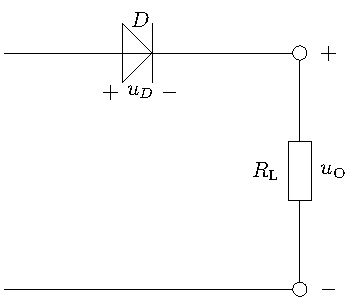
\includegraphics[width=0.5\textwidth]{tu6}
			\caption{示意图}\label{tu:6}
		\end{figure}
	\item (17)一台三相四极笼型异步电动机, 额定功率 $P_{\NN}=10\zt{kW}$ , 额定电压 $U_{1\NN}=380\zt{V}$ , 额定转速 $n_{\NN}=1460\zt{r/min}$ , 额定频率 $f_{1\NN}=50\zt{Hz}$ , 三角形连接, 每相参数为 $R_1=1.35\Omega$ , $X_{1\sigma}=2.43\Omega$ , $R_2'=1.35\Omega$ , $X_{2\sigma}'=4.5\Omega$ , $R_{\mathrm{m}}=7.2\Omega$ , $X_{\mathrm{m}}=92\Omega$ , 试用 $\Gamma$  型等效电路计算电机在额定运行时的定子相电流 $\dot{I}_{1\NN}$ 、功率因数 $\cos\varphi_{1\NN}$ 和效率 $\eta_{\NN}$ .\daan{js:27}
	\item (17)某四极直流电机, 电枢槽数 $Z=36$ , 单叠绕组, 每槽导体数为 $6$ , 每极磁通 $2.1\times 10^{-2}\zt{Wb}$ , 电枢电流 $I_a=820\zt{A}$ ,  问此时电磁转矩为多少? 如改为单波绕组, 保持支路电流不变, 其电磁转矩为多少?\daan{js:28}
	\item (17)某四极他励直流电动机电枢绕组为单波, 电枢总导体数 $N=372$ , 电枢回路的总电阻 $R=0.21\Omega$ , 运行于 $U=220\zt{V}$ 的直流电网并测得转速 $n=1460\zt{r/min}$ , 每极磁通 $\varPhi=0.011\zt{Wb}$ , 铁耗 $p_{\mathrm{Fe}}=362\zt{W}$ , 机械损耗 $p_{\Omega}=204\zt{W}$ , 附加损耗忽略不计, 试问:
		\begin{enumerate}
			\item 此时该机是运行于发电机状态还是电动机状态?
			\item 电磁功率与电磁转矩为多少?
			\item 输入功率与效率为多少?\daan{js:29}
		\end{enumerate}
	\item (17)一台他励直流电动机, 额定数据为: $P_{\NN}=102\zt{kW}$ , $I_{\NN}=526\zt{A}$ , $U_{\NN}=220\zt{V}$ , $n_{\NN}=1250\zt{r/min}$ , 电枢回路总电阻 $R_a=0.048\Omega$ , 求:
		\begin{enumerate}
			\item 额定负载时的电枢电动势 $E_{a\NN}$ 和额定电磁转矩 $T_{\NN}$ .
			\item 额定轴上输出转矩 $T_{2\NN}$ 和空载转矩 $T_0$ .
			\item 理想空载转速 $n_0$ 和实际空载转速 $n_0'$ .\daan{js:30}
		\end{enumerate}
	\item (17)三相四极异步电动机 $P_{\NN}=2.9\zt{kW}$ , $U_{1\NN}=380\zt{V}$ , 三角形连接, $n_{\NN}=1450\zt{r/min}$ , 定子参数为: 每相绕组串联匝数 $N_1=250$ 匝, 绕组系数 $k_{N1}=0.955$ , $R_1=1.85\Omega$ , $X_{1\sigma}=2.2\Omega$ . 转子参数为: 槽数 $Z_2=44$ , $R_2=1.2\times 10^{-4}\Omega$ , $X_{2\sigma}=1.42\times 10^{-4}\Omega$ . 励磁参数为: $R_{\mathrm{m}}=7.4\Omega$ , $X_{\mathrm{m}}=96\Omega$ , 试求:
		\begin{enumerate}
			\item 转子参数折算值 $R_2'$ , $X_{2\sigma}'$ .
			\item 画出其 $\Gamma$ 形简化等值电路.
			\item 用 $\Gamma$ 形简化等值电路计算定子相电流 $I_{1\varphi}$ 及定子额定线电流 $I_{1\NN}$ .\daan{js:31}
		\end{enumerate}
\end{enumerate}





\chapter{电机题库答案}
\section{填空题答案}
\begin{enumerate}
	\item \label{tk:1}他励、并励、串励、复励.
	\item \label{tk:2}交变、直流.
	\item \label{tk:3}能耗、反接、回馈、电压、电动势.
	\item \label{tk:4}定子串电抗器、自耦变压器、 $\zt{Y}-\triangle$ 、延边 $\triangle$ .
	\item \label{tk:5}励磁电抗、励磁电阻、励磁阻抗.
	\item \label{tk:6}增大、不变、增大、下降、增大.
	\item \label{tk:7}圆形旋转、交变.
	\item \label{tk:8}主磁通、过载能力.
	\item \label{tk:9} $\frac{1}{3}$
	\item \label{tk:10}电机应有剩磁、励磁绕组连接正确、磁场回路电阻应小于临界电阻.
	\item \label{tk:11}单叠绕组、单波绕组、负载电流大, 感应电动势小、负载电流小, 感应电动势大.
	\item \label{tk:12} $U=U_{\NN}$ 、 $\varPhi=\varPhi_{\NN}$ 、电阻、 $n$ 、 $T_{\zt{em}}$ .
	\item \label{tk:13}电枢回路串电阻启动、降压/\elegantpar{控硅}{近代广泛采用可控硅整流电源}启动.
	\item \label{tk:14}理想空载转速.
	\item \label{tk:15}圆形旋转、三相电流相位、同步转速 $n=\frac{60f}{p}$ .
	\item \label{tk:16}总机械功率.
	\item \label{tk:17} $(0,s_{\mathrm{m}})$ .
	\item \label{tk:18}电流的趋肤效应.
	\item \label{tk:19}电枢电压极性、励磁绕组方向.
	\item \label{tk:20}降压调速、弱磁调速.
	\item \label{tk:21}相反、相同.
	\item \label{tk:22}电源电压、材质、几何尺寸、磁化曲线.
	\item \label{tk:23}转速、幅值、方向.
	\item \label{tk:24}临界转矩与额定电磁转矩的比值.
	\item \label{tk:25}电枢.
	\item \label{tk:26}系统机械惯量的大小.
	\item \label{tk:27}减小电机启动时对电网的冲击电流.
	\item \label{tk:28}励磁阻抗大.
	\item \label{tk:29}反转.
	\item \label{tk:30} $P_1=P_2+p_{\zt{Cu}1}+p_{\mathrm{Fe}}+p_{\zt{Cu}2}+p_{\mathrm{mec}}+p_{\zt{ad}}$ 、 $T_{\zt{em}}=T_2+T_0$ .
	\item \label{tk:31}\begin{equation*}
		\begin{cases}
			\dot{U}_1=-\dot{E}_1+\dot{I}_1 Z_1\\
			\dot{E}_2'=\dot{I}_2'\left( \frac{R_2'}{s}+\zt{j}X_{2\sigma}' \right)\\
			\dot{I}_1=\dot{I}_0-\dot{I}_2'\\
			\dot{E}_1=\dot{E}_2'\\
			\dot{E}_1=-\dot{I}_0Z_{\mathrm{m}}
		\end{cases}
	\end{equation*}
	\item \label{tk:32}参考填空题~\ref{tk:28}~的答案.
	\item \label{tk:33}
	\item \label{tk:34}
	\item \label{tk:35}参考填空题~\ref{tk:36}~的答案.
	\item \label{tk:36}
	\item \label{tk:37}
	\item \label{tk:38}不能空载或者负载很小、励磁绕组不能开路.
	\item \label{tk:39}恒转矩、恒转矩.
	\item \label{tk:40}
	\item \label{tk:41}
	\item \label{tk:42}
	\item \label{tk:43}
	\item \label{tk:44}
	\item \label{tk:45}
	\item \label{tk:46}
	\item \label{tk:47}
	\item \label{tk:48}
	\item \label{tk:49}
	\item \label{tk:50}
	\item \label{tk:51}
	\item \label{tk:52}
	\item \label{tk:53}
	\item \label{tk:54}
	\item \label{tk:55}
	\item \label{tk:56}
	\item \label{tk:57}
	\item \label{tk:58}
	\item \label{tk:59}
	\item \label{tk:60}
	\item \label{tk:61}
	\item \label{tk:62}
	\item \label{tk:63}
	\item \label{tk:64}
	\item \label{tk:65}
	\item \label{tk:66}
	\item \label{tk:67}
	\item \label{tk:68}
	\item \label{tk:69}
	\item \label{tk:70}
	
\end{enumerate}
\section{画图题答案}
\begin{enumerate}
	\item \label{ht:1}此题答案详见计算题~\ref{js:1}~.
	\item \label{ht:2}机械特性曲线见图~\ref{tu:5}~
		\begin{figure}[htbp]
			\centering
			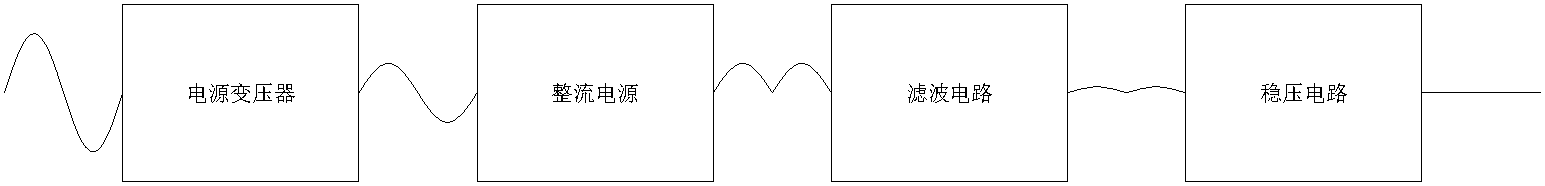
\includegraphics[width=0.5\textwidth]{tu5}
			\caption{异步电动机的机械特性曲线}\label{tu:5}
		\end{figure}
	\item \label{ht:3}
	\item \label{ht:4}
	\item \label{ht:5}能流图见图~\ref{tu:3}~.
		\begin{figure}[htbp]
			\centering
			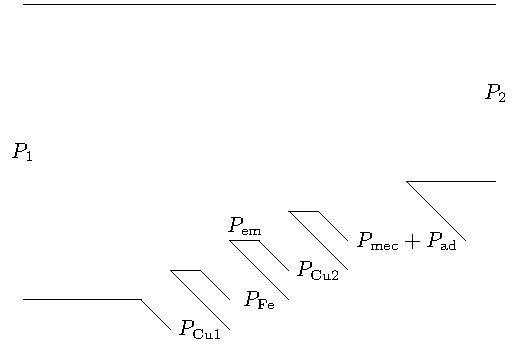
\includegraphics[width=0.8\textwidth]{tu3}
			\caption{三相感应电动机的能流图}\label{tu:3}
		\end{figure}
\end{enumerate}

\section{计算题答案}
\begin{enumerate}
	\item \label{js:1}一台他励直流电动机, 铭牌数据如下: $P_{\NN}=60\zt{kW}, U_{\NN}=220\zt{V}, I_{\NN}=305\zt{A}, n_{\NN}=1000\zt{r/min}$ . 试求:
		\begin{enumerate}
			\item 固有机械特性.
			\item $R_{C}=0.5\Omega$ 的人为机械特性.
		\end{enumerate}
			\begin{solution}
				\begin{enumerate}
					\item 固有机械特性
						\begin{enumerate}
							\item 估算电枢电阻 $R_{a}$
								\begin{equation*}
									R_{a}\approx \frac{1}{2}\left(\frac{U_{\NN} I_{\NN}-P_{\NN}}{I_{\NN}^{2}}\right)=\frac{1}{2}\left(\frac{220 \times 305-60 \times 10^{3}}{305^{2}}\right)=0.038 \Omega
								\end{equation*}
							\item 计算 $C_{E}\varPhi_{\NN}$
								\begin{equation*}
									\elegantpar{C_{E}\varPhi_{\NN}=\frac{U_{\NN}-I_{\NN}R_{a}}{n_{\NN}}}{ref: 课本 P65 式(2.30)}=\frac{220-305 \times 0.038}{1000}=0.2084\zt{V(r/min)}^{-1}
								\end{equation*}
							\item 理想空载转速 $n_0$
								\begin{equation*}
									n_0=\frac{U_{\NN}}{C_{E}\varPhi_{\NN}}=\frac{220}{0.2084}=1056\zt{r/min}
								\end{equation*}
							\item 额定电磁转矩 $T_{\NN}$
								\begin{equation*}
									\elegantpar{T_{\NN}=9.55 C_{E} \varPhi_{\NN} I_{\NN}}{由 $T=\frac{P}{\Omega}$ 化简可得} =9.55 \times 0.2084 \times 305=607\zt{N\cdot m}
								\end{equation*}
								注: 理想空载点( $n_0=1056\zt{r/min}$ , $T=0$ ), 额定运行点( $n=n_{\NN}=1000\zt{r/min}$ , $T_{\NN}=607\zt{N\cdot m}$ ), 绘出固有机械特性, 如图~\ref{tu:2}~中的直线 $1$ .
						\end{enumerate}
					\item $R_C=0.5\Omega$ 的人为机械特性
						\begin{enumerate}
							\item 理想空载转速 $n_0=1056\zt{r/min}$
							\item $T=T_{\NN}$ 时电动机的转速 $n_{R\NN}$
								\begin{equation*}
									\elegantpar{n_{R\NN}=n_0-\frac{R_a+R_C}{9.55( C_E \varPhi_{\NN})^2}T_{\NN}}{ref: 课本 P79 式(2.73)}=1056-\frac{0.038+0.5}{9.55 \times 0.2084^{2}} \times 607=268\zt{r/min}
								\end{equation*}
								通过( $n_0=1056\zt{r/min}$ , $T=0$ )及( $n=n_{R\NN}=268\zt{r/min}$ , $T_{\NN}=607\zt{N\cdot m}$ )两点连一直线, 即得 $R_C=0.5\Omega$ 的人为机械特性, 如图~\ref{tu:2}~直线 $2$ .
						\end{enumerate}
				\end{enumerate}
				\begin{figure}[htbp]
					\centering
					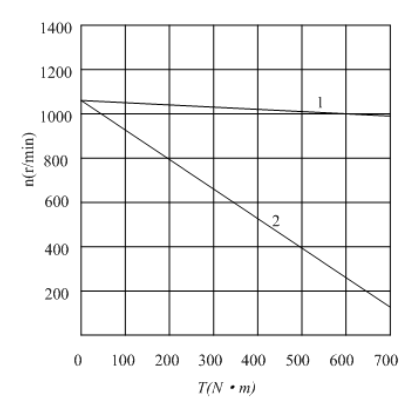
\includegraphics[width=0.4\textwidth]{tu2}
					\caption{机械特性曲线}\label{tu:2}
					\quad
					\parbox[b]{0.4\textwidth}{
					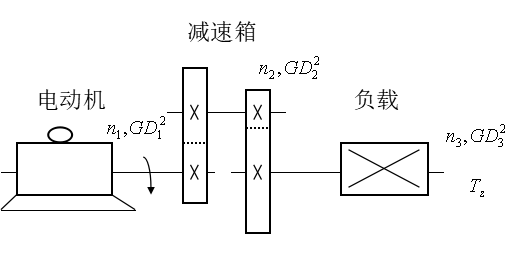
\includegraphics[width=0.5\textwidth]{tu4}}
			\caption{传动机构图}\label{tu:7}
				\end{figure}
			\end{solution}
	\item \label{js:2}电力拖动系统的传动机构如图~\ref{tu:7}~所示, 已知: $n_1=2500\zt{r/min}$ , $n_2=1000\zt{r/min}$ , $n_3=500\zt{r/min}$ , $GD_1^2=8\zt{kg\cdot m^2}$ , $GD_2^2=25\zt{kg\cdot m^2}$ , $GD_3^2=75\zt{kg\cdot m^2}$ , 负载转矩 $T_Z=10\zt{kg\cdot m}$ , 电磁转矩 $T=3\zt{kg\cdot m}$ , 试求:
		\begin{enumerate}
			\item 生产机械轴的平均加速度为多少?
			\item 要加装 $62.5\zt{kg\cdot m^2}$ 的飞轮, 以使生产机械轴的平均加速度为 $3 \zt{r/(min\cdot s)}$ , 此飞轮应装在哪个轴合适?
		\end{enumerate}
		% \begin{figure}[htbp]
		% 	\centering
			
		% \end{figure}
		\begin{solution}
			$j_2=\frac{n_1}{n_2}=\frac{2500}{1000}=2.5$ , $j_3=\frac{n_1}{n_3}=\frac{2500}{500}=5$
			\begin{enumerate}
				\item 折算到电机轴上的负载转矩
					\begin{align*}
						&T_Z'=\frac{T_Z}{j_3}=\frac{T_Z}{\frac{n_1}{n_3}}=\frac{10}{\frac{2500}{500}}=2\zt{kg\cdot m}\\
						&GD_{zc}^2=GD_1^2+\frac{GD_2^2}{j_2^2}+\frac{GD_3^2}{j_3^2}=8+\frac{25}{2.5^2}+\frac{75}{5^2}=15\zt{kg\cdot m^2}
					\end{align*}
					由 $T=T_Z'+\frac{GD_{zc}^2}{375}\frac{\dd n}{\dd t}$ (推导见旁注~\ref{pz:1}~\footnote{这里的交叉引用并不准确})可得
					\begin{equation*}
						\frac{\dd n}{\dd t}=\frac{375(T-T_{z}')}{GD_{zc}^2}=\frac{375(3-2)}{15}=25\zt{r/(min\cdot s)}
					\end{equation*}
					负载轴加速度
					\begin{equation*}
						\frac{\dd n_z}{\dd t}=\frac{\frac{\dd n}{\dd t}}{j_3}=\frac{25}{5}=5\zt{r/(min\cdot s)}
					\end{equation*}
				\item 由题可知 $\frac{\dd n_z}{\dd t}=3\zt{r/(min\cdot s)}$ , 可得:
				\begin{align*}
					&\frac{\dd n}{\dd t}=j_3\frac{\dd n_z}{\dd t}=5\frac{\dd n_z}{\dd t}=\frac{375(T-T_z')}{GD_{zc}^2+GD_x^2}\\
					&GD_{x}^2=\frac{375\times 1}{5\times 3}-GD_{zc}^2=25-15=10\zt{kg\cdot m^2}\\
					&j_x^2=\frac{\triangle GD^2}{GD_x^2}=\frac{62.5}{10}=6.25\\
					&j_x=2.5
				\end{align*}
				所以应加在第二轴.
			\end{enumerate}
		\end{solution}
	\item \label{js:3}一台他励直流电动机, 额定数据为: $P_{\NN}=1.1\zt{kW}$ , $U_{\NN}=110\zt{V}$ , $I_{\NN}=13\zt{A}$ , $n_{\NN}=1500\zt{r/min}$ , 电枢回路电阻 $R_a=1\Omega$ . 计算:
		\begin{enumerate}
			\item 额定电磁转矩.
			\item 额定输出转矩.
			\item 空载转矩.
			\item 理想空载转速.
			\item 实际空载转速.
		\end{enumerate}
		\begin{solution}
			\begin{enumerate}
				\item 额定电磁转矩 $\elegantpar{T_{\mathrm{em}}=\frac{P_{\NN}}{\Omega_{\NN}}}{这个公式比起 $E=C_{E}\varPhi n$ 和 $T_{\mathrm{em}}=C_{T}\varPhi I_a$ 是容易记忆的}=\frac{30(U_{\NN}-I_{\NN}R_a)I_{\NN}}{\uppi n_{\NN}}=\frac{30 (110-13\times 1)\times 13}{1500\uppi}=8.03\zt{N\cdot m}$
				\item 额定输出转矩 $T_{2\NN}=\frac{P_{\NN}}{\Omega_{\NN}}=\frac{30P_{\NN}}{\uppi n}=\frac{30\times 1100}{1500\uppi}=7.00\zt{N\cdot m}$
				\item 空载转矩 $T_0=T_{\mathrm{em}}-T_{2\NN}=8.03-7=1.03\zt{N\cdot m}$
				\item 理想空载转速 $n_0=\frac{U_{\NN}}{C_{E}\varPhi_{\NN}}=\frac{U_{\NN}}{\frac{U_{\NN}-I_{\NN}R_a}{n_{\NN}}}=\frac{110\times 1500}{110-13\times 1}=1701.03\zt{r/min}$
				\item 实际空载转速
				\begin{align*}
					n_0'&=\frac{U_{\NN}-I_{a}R_a}{C_{E}\varPhi_{\NN}}=n_{\NN}\frac{U_{\NN}-I_{a}R_a}{U_{\NN}-I_{\NN}R_a}=n_{\NN}\frac{U_{\NN}-I_{\NN}\frac{T_0}{T_{\mathrm{em}}}R_a}{U_{\NN}-I_{\NN}R_a}\\
					&= 1500\times\frac{110-13\times\frac{1.03}{8.03}\times 1}{110-13} = 1675.24\zt{r/min}
				\end{align*}
			\end{enumerate}
		\end{solution}

	\item \label{js:4}一台他励直流电动机数据为: $P_{\NN}=7.5\zt{kW}$ , $U_{\NN}=110\zt{V}$ , $I_{\NN}=79.84\zt{A}$ , $n_{\NN}=1500\zt{r/min}$ , 电枢回路电阻 $R_a=0.1014\Omega$ , 求:
		\begin{enumerate}
			\item $U=U_{\NN}$ , $\varPhi=\varPhi_{\NN}$ 条件下, 电枢电流 $I_a=60\zt{A}$ 时转速是多少?
			\item $U=U_{\NN}$ 条件下, 主磁通减少 $15\%$ , 负载转矩为 $T_{\NN}$ 不变时, 电动机电枢电流与转速是多少?
			\item $U=U_{\NN}$ , $\varPhi=\varPhi_{\NN}$ 条件下, 负载转矩为 $0.8T_{\NN}$ , 转速为 $800\zt{r/min}$ , 电枢回路应串入多大电阻?
		\end{enumerate}
		\begin{solution}
			\begin{enumerate}
				\item $n_a=\frac{U_{\NN}-I_{a}R_a}{C_E\varPhi_{\NN}}=\frac{U_{\NN}-I_{a}R_a}{\elegantpar{\frac{U_{\NN}-I_{\NN}R_a}{n_{\NN}}}{这里可以求出 $C_{E}\varPhi_{\NN}=0.068$ }}=1500\times\frac{110-60\times 0.1014}{110-79.84\times 0.1014}=1529.61\zt{r/min}$
				\item $\elegantpar{I=\frac{T}{C_T\varPhi}}{ref: 课本 P65 式(2.34)}=\frac{T_{\NN}}{0.85C_T \varPhi_{\NN}}=1.18 I_{\NN}=1.18\times 79.84=94.21\zt{A}$
				
					$n=\frac{U_{\NN}-IR_a}{C_E \varPhi_{\NN}}=\frac{110-94.21\times 0.1014}{0.068}=1477.16\zt{r/min}$
				\item $I=\frac{T}{C_T \varPhi_{\NN}}=\frac{0.8T_{\NN}}{C_T \varPhi_{\NN}}=0.8I_{\NN}=0.8\times 79.84=63.872\zt{A}$
				
				$n=\frac{U_{\NN}-I(R_a+R_x)}{C_E \varPhi_{\NN}}=\frac{110-63.872(0.1014+R_x)}{0.068}=800$

				解得 $R_x=0.77\Omega$
			\end{enumerate}
		\end{solution}
	\item \label{js:5}一台 $S_{\NN}=100\zt{kV\cdot A}$ , $U_{1\NN}/U_{2\NN}=6/0.4\zt{kV}$ , $\mathrm{Yy}0$ 连接的三相变压器, $I_0^*=6.5\% $ , $P_0=600\zt{W}$ , $u_{S_{\NN}}^*=5\%$ , $P_{S_{\NN}}=1800\zt{W}$ , 试求:
	\begin{enumerate}
		\item 近似等效电路参数标么值.
		\item 满载及 $\cos\varPhi_2=0.8(\text{滞后})$ 时的二次端电压和效率.
		\item 产生最大效率时的负载电流及 $\cos\varPhi_2=0.8(\varPhi_2>0^\circ)$ 时的最大效率.
	\end{enumerate}
	\item \label{js:6}
	\item \label{js:7}
	\item \label{js:8}
	\item \label{js:9}
	


	\item \label{js:10}他励直流电动机额定数据为: $P_{\NN}=29\zt{kW}$ , $U_{\NN}=440\zt{V}$ , $I_{\NN}=76\zt{A}$ , $n_{\NN}=1000\zt{r/min}$ , $R_a=0.377\Omega$ . 求:
	\begin{enumerate}
		\item 该机以 $300\zt{r/min}$ 的速度吊起 $T_Z=0.8T_{\NN}$ 的负载转矩, 在电枢回路应串多大电阻?
		\item 用能耗制动的方法使 $T_Z=0.8T_{\NN}$ 的位能负载以 $400\zt{r/min}$ 的速度稳速下放, 在电枢回路应串多大电阻?
	\end{enumerate}
	\begin{solution}
		根据电压平衡式可求得额定运行时:
		\begin{equation*}
			E_{a\NN}=U_{\NN}-I_aR_a=440-76\times 0.377=411.35\zt{V}
		\end{equation*}
		\begin{enumerate}
			\item $n=300\zt{r/min}$ , $T_Z=0.8T_{\NN}$ 时, $E_a=0.3\times 411.35=123.405\zt{V}$ , $I_a=0.8I_{\NN}=0.8\times 76=60.8\zt{A}$
				\begin{equation*}
					R_Z=\frac{U_{\NN}-E_a}{I_a}-R_a=\frac{440-123.405}{60.8}-0.377=4.83\Omega
				\end{equation*}
		\end{enumerate}
	\end{solution}





	\item \label{js:11}
	




	\item \label{js:12}某三相绕线式感应电动机的额定数据如下: $P_{\NN}=7.5\zt{kW}$ , $U_{\NN}=380\zt{V}$ , $I_{\NN}=15.1\zt{A}$ , $n_{\NN}=1450\zt{r/min}$ , $\lambda_{M}=2$ . 现将定子线电压降为 $220\zt{V}$ , 试求:
	\begin{enumerate}
		\item 降压后人为特性的实用表达式.
		\item 降压后的起动转矩? 这时该机能否满载起动? 为什么?
		\item 降压后的过载能力?
	\end{enumerate}
	\begin{solution}
		\begin{enumerate}
			\item 
			\item 
			\item 
		\end{enumerate}
	\end{solution}
	\item \label{js:13}
	\item \label{js:14}
	\item \label{js:15}
	\item \label{js:16}
	\item \label{js:17}
	\item \label{js:18}
	\item \label{js:19}
	\item \label{js:20}
	\item \label{js:21}
	\item \label{js:22}
	\item \label{js:23}
	\item \label{js:24}
	\item \label{js:25}
	\item \label{js:26}某车床电力拖动系统中, 已知切削力 $F=1950\zt{N}$ , 工件直径 $d=155\zt{mm}$ , 电动机转速为 $1460\zt{r/min}$ ,  减速箱三级速比 $j_1=2$ , $j_2=1.5$ , $j_3=2$ , 各转轴飞轮矩为 $GD_1^2=3.2\zt{N\cdot m^2}$ (电动机轴), $GD_2^2=2.5\zt{N\cdot m^2}$ , $GD_3^2=2.8\zt{N\cdot m^2}$ , $GD_4^2=8.5\zt{N\cdot m^2}$ , 各级传动效率 $\eta_1=\eta_2=\eta_3=0.88$ , 求:
		\begin{enumerate}
			\item 切削功率.
			\item 电动机输出功率.
			\item 系统总飞轮矩.
			\item 忽略电动机空载转矩时, 电动机电磁转矩.
			\item 车床开车未切削时, 若电动机加速度 $\frac{\dd n}{\dd t}=820\zt{r/(min\cdot s)}$ , 忽略电动机空载转矩, 但不忽略传动机构转矩损耗, 求电动机电磁转矩.
		\end{enumerate}
		\begin{solution}
			$n_z=\frac{n}{j_1j_2j_3}=\frac{1460}{2\times 1.5\times 2}=243.33\zt{r/min}$
			\begin{enumerate}
				\item 工件边缘的旋转速率 $v=\Omega_z\frac{d}{2}=\frac{\uppi n_z}{30}\frac{d}{2}=\frac{243.33\uppi}{30}\frac{0.155}{2}=1.97\zt{m/s}$ , 则切削功率 $P_L = Fv = 1950\times 1.98=3850.89\zt{W}$
				\item 电机输出功率 $P_2=\frac{P_L}{\eta_1\eta_2\eta_3}=\frac{3850.89}{0.88^3}=5650.84\zt{W}$
				\item 系统总飞轮矩 $\elegantpar{GD^2=GD_1^2+\frac{GD_2^2}{j_2^2}+\frac{GD_3^2}{j_1^2j_2^2}+\frac{GD_4^2}{j_1^2j_2^2j_3^2}}{由 $J=\sum_{k=0}^n J_k \left( \frac{\Omega_k}{\Omega_0} \right)^2$\footnote{ref: 课本 P81 式(2.82)} 可推得}=3.2+\frac{2.5}{2^2}+\frac{2.8}{2^2\cdot 1.5^2}+\frac{8.5}{2^2\cdot 1.5^2\cdot 2^2}=4.37\zt{N\cdot m^2}$
				\item 电动机电磁转矩 $T_2=\frac{P_2}{\Omega_2}=\frac{P_L}{\eta_1\eta_2\eta_3}\frac{30}{\uppi n}=\frac{3850.89\times 30}{0.88^3 \times 1460 \uppi }=36.96\zt{N\cdot m}$
				\item 忽略损耗时的电动机电磁转矩 $T_2'=\frac{P_L}{\Omega_2}=\frac{30P_L}{\uppi n}=\frac{3850.89\times 30}{1460\uppi}=25.19\zt{N\cdot m}$ , 那么传动机构转矩损耗 $T_0=T_2-T_2'=36.96-25.19=11.77\zt{N\cdot m}$ , 加速时电动机转矩 $\elegantpar{\label{pz:1}T_{\mathrm{em}}=T_0+\frac{GD^2}{375}\frac{\dd n}{\dd t}}{由实用方程 $J=\frac{GD^2}{4g}$\footnote{ref: 课本 P80 式(2.78)} 、 转子运动方程 $J\frac{\dd \Omega}{\dd t}=T_{\mathrm{em}}-T_{\mathrm{L}}$\footnote{ref: 课本 P80 式(2.77)} 及 $\Omega=\frac{\uppi}{30}n$ 推出}=11.77+\frac{4.37}{375}\times 820=21.33\zt{N\cdot m}$
			\end{enumerate}
		\end{solution}

	\item \label{js:27}
	\item \label{js:28}
	\item \label{js:29}
	\item \label{js:30}
	\item \label{js:31}

\end{enumerate}


\bibliography{reference}
\end{document}